\everymath{\displaystyle}

%%%%%%%%%%%%%%%%%%%%%%%%%%%%%%%%%%%%%%%%
%           main body
%%%%%%%%%%%%%%%%%%%%%%%%%%%%%%%%%%%%%%%%

%-----------------------------------
%	TITLE PAGE
%-----------------------------------

\title[第三章\\
可测函数]{\texorpdfstring{\LARGE \bfseries 第三章\quad 可测函数}{第三章 可测函数}}
\author[\S 3.1\\
可测函数的基本性质]
{\Large \bfseries \S 3.1 可测函数的基本性质}
\date{}

%------------------------------------------------

\begin{document}

%------------------------------------------------

\begin{frame}

\titlepage

\end{frame}

%------------------------------------------------

\section{引言}

%------------------------------------------------

\begin{frame}{回顾: Lebesgue 积分的想法}

第二章结尾留下的问题: 按\alert{分割值域}的思路定义积分. 设 $f: [a,b] \to [m, M]$, 取值域分割
\[
\Delta:\ m = y_0 < y_1 < \cdots < y_n = M,
\qquad
E_k = \{x:\ y_{k-1} \leqslant f(x) < y_k\},
\]
令 $\lambda(\Delta) \to 0$,
\[
\int_{[a,b]} f(x)\,\mathrm{d}x \ ``=" \lim \sum_{k=1}^{n} y_{k-1}\, m E_k .
\]

\pause

\begin{question}
公式里的 $mE_k$ 已经就绪 (第二章), 但 $E_k$ 本身\alert{可测吗}? 什么样的 $f$ 保证这些水平集可测?
\end{question}

\pause

\textbf{本章任务}: 挑出``好的''函数 --- \alert{可测函数}; 研究其运算、极限 (\S 3.1) 与各种收敛性 (\S 3.2), 并刻画其构造 (\S 3.3, Luzin 定理).

\end{frame}

%------------------------------------------------

\section[定义]{可测函数的定义}

%------------------------------------------------

\begin{frame}{可测函数的定义}

\begin{Def}[可测函数]
设 $f$ 是定义在\alert{可测集} $E \subset \mathbb{R}$ 上的\alert{扩充实值}函数 ($f: E \to \mathbb{R} \cup \{\pm\infty\}$). 若 $\forall\, \alpha \in \mathbb{R}$, 集合
\[
E(f > \alpha) := \{x \in E:\ f(x) > \alpha\} = f^{-1}\big((\alpha, +\infty]\big)
\]
都是 (勒贝格) 可测集, 则称 $f$ 为 $E$ 上的\alert{(勒贝格) 可测函数}.
\end{Def}

\pause

\begin{remark}[等价的水平集族]
定义中的 $E(f > \alpha)$ 可替换为
\[
E(f \geqslant \alpha) = \bigcap_{k=1}^\infty E\big(f > \alpha - \tfrac{1}{k}\big), \quad
E(f < \alpha),\ E(f \leqslant \alpha),\ E(f = +\infty) = \bigcap_{n=1}^\infty E(f > n),
\]
以及 $E(\alpha < f < \beta) = E(f > \alpha) \cap E(f < \beta)$ 等 ($-\infty$ 情形同理) --- 可测集类对\alert{可数交、并、差、补}封闭 (§2.3).
\end{remark}

\begin{remark}
$f$ 连续 $\implies$ $f$ 可测: $E(f > \alpha) = f^{-1}\big((\alpha, +\infty)\big) \cap E$ 是开集与 $E$ 的交 (§1.3: 连续 $\iff$ 开集的原像为开). \alert{可测函数是连续函数的巨大扩张}.
\end{remark}

\end{frame}

%------------------------------------------------

\begin{frame}{第一个例子: Dirichlet 函数}

\begin{eg}[Dirichlet 函数]
$E = [0, 1]$, $D(x) = \chi_{\mathbb{Q} \cap [0,1]}(x)$. 逐段验证 $E(D > \alpha)$:
\[
\alpha < 0:\ E(D>\alpha) = [0,1] = E;
\qquad
0 \leqslant \alpha < 1:\ E(D>\alpha) = \mathbb{Q} \cap [0,1];
\qquad
\alpha \geqslant 1:\ E(D>\alpha) = \emptyset.
\]
三者皆可测 (零测集的子集可测), 故 $D$ 是\alert{可测函数}.
\end{eg}

\pause

\begin{attnblock}
$D$ 在\alert{每一点都不连续}, Riemann 意义下不可积; 但它是可测函数 --- 可测性对函数的要求\alert{非常宽松}, 这正是勒贝格理论威力之源.
\end{attnblock}

\pause

\begin{remark}
直观: ``$f$ 可测'' $\iff$ 定义域 $E$ 被诸水平集 $E(f>\alpha)$ \alert{不搞得乱七八糟} (每个都测得到) --- 值域的分割片 $E_k = E(y_{k-1} \leqslant f < y_k)$ 都可测, 积分公式才有意义.
\end{remark}

\end{frame}

%------------------------------------------------

\section{简单函数}

%------------------------------------------------

\begin{frame}{简单函数}

\begin{Def}[简单函数]
设 $f: E \to \mathbb{R}$, $E$ 可测, $f(E) = \{c_1, c_2, \ldots, c_n\}$ 有限, 且诸水平集 $E(f = c_i)$ 都可测, 则
\[
f = \sum_{i=1}^{n} c_i\, \chi_{E(f = c_i)}
\]
称为 $E$ 上的\alert{简单函数} (可测集特征函数的有限线性组合).
\end{Def}

\begin{eg}
Dirichlet 函数 $D = 1 \cdot \chi_{\mathbb{Q} \cap [0,1]} + 0 \cdot \chi_{[0,1] \setminus \mathbb{Q}}$ 是简单函数.
\end{eg}

\pause

\begin{lem}[简单函数可测]
简单函数都是可测函数.
\end{lem}

\startproof[bg=yellow, fg=red](证明)
不妨设 $c_1 < c_2 < \cdots < c_n$. $\forall\, \alpha \in \mathbb{R}$:
\[
\alpha \geqslant c_n:\ E(f>\alpha) = \emptyset; \qquad
c_k \leqslant \alpha < c_{k+1}:\ E(f>\alpha) = \bigcup_{i=k+1}^{n} E(f = c_i); \qquad
\alpha < c_1:\ E(f>\alpha) = E.
\]
右端皆可测.
\qed

\pause

\begin{remark}
简单函数是可测函数中结构最简单的一类, 后面它会\alert{逼近一般可测函数} (\S 3.1 末) 并充当积分的积木 (\S 4.1), 也能简化许多证明 (包括习题).
\end{remark}

\end{frame}

%------------------------------------------------

\section[验证技巧]{可测性的验证: 稠密集、限制与拼接}

%------------------------------------------------

\begin{frame}{稠密集判别法}

\begin{thm}[稠密集判别法]
设 $f: E \to \mathbb{R}$ ($E$ 可测), $D \subset \mathbb{R}$ 是\alert{稠密集}. 若 $\forall\, \alpha \in D$, $E(f > \alpha)$ 都可测, 则 $f$ 是可测函数.
\end{thm}

\startproof[bg=yellow, fg=red](证明)
$\forall\, \gamma \in \mathbb{R}$, 由 $D$ 稠密, 可取 $D$ 中点列 $\alpha_1, \alpha_2, \ldots$ 使 $\alpha_k > \gamma$ 且 $\alpha_k \to \gamma$. 断言:
\[
E(f > \gamma) = \bigcup_{k=1}^{\infty} E(f > \alpha_k).
\]
``$\supset$''显然. ``$\subset$'': 任取 $x \in E(f>\gamma)$, 即 $f(x) > \gamma$, 由 $\alpha_k \to \gamma$ 可找到 $\alpha_{k_0} \leqslant f(x)$, 故 $x \in E(f > \alpha_{k_0})$.

于是 $E(f>\gamma)$ 是可列个可测集之并, 可测.
\qed

\pause

\begin{remark}
取 $D = \mathbb{Q}$: 可列 $+$ 稠密, 只需验证\alert{可列多个}水平集 --- 定义里的``$\forall\, \alpha \in \mathbb{R}$''常常可以减负.
\end{remark}

\end{frame}

%------------------------------------------------

\begin{frame}{限制与拼接}

\begin{thm}[拼接]
设 $f$ 是 $E_1 \cup E_2$ 上的扩充实值函数, $E_1, E_2$ 可测. 若 $f\big|_{E_1}$ 与 $f\big|_{E_2}$ 都可测, 则 $f$ 在 $E_1 \cup E_2$ 上可测.
\end{thm}

\startproof[bg=yellow, fg=red](证明)
\[
E(f > \alpha) = \{x \in E_1:\ f(x) > \alpha\} \cup \{x \in E_2:\ f(x) > \alpha\}
= E\big(f\big|_{E_1} > \alpha\big) \cup E\big(f\big|_{E_2} > \alpha\big).
\]
\qed

\pause

\begin{thm}[限制]
若 $f: E \to \mathbb{R}$ 可测, $A \subset E$ 为可测集, 则 $f\big|_A: A \to \mathbb{R}$ 可测.
\end{thm}

\startproof[bg=yellow, fg=red](证明)
\[
E\big(f\big|_A > \alpha\big) = A \cap E(f > \alpha).
\]
\qed

\pause

\begin{remark}
可测性在定义域的\alert{限制}与\alert{拼接}下不变: 分段 (各段可测) 定义的函数可测.
\end{remark}

\end{frame}

%------------------------------------------------

\section{几乎处处}

%------------------------------------------------

\begin{frame}{几乎处处 (a.e.)}

\begin{Def}[几乎处处]
设 $S$ 是关于集 $E$ 的某个命题 (性质). 若存在\alert{零测集} $Z$, 使得 $S$ 在 $E \setminus Z$ 上处处成立, 则称 $S$ 在 $E$ 上\alert{几乎处处}成立 (almost everywhere, 简记 a.e.).

特别地, 若 $f = g$ a.e.\ 于 $E$, 称 $f$ 与 $g$ \alert{对等}, 记作 $f \sim g$.
\end{Def}

\pause

\begin{eg}
Dirichlet 函数 $D = 0$ a.e.\ 于 $[0,1]$: 例外集 $\mathbb{Q} \cap [0,1]$ 是零测集.
\end{eg}

\pause

\begin{remark}
\begin{itemize}
\item 例外集可以``很大'': Cantor 集 $P_0$ 零测但具有连续统的势 --- a.e.\ 只看\alert{测度}, 不看点数;
\item a.e.\ 成立的命题可以换一个零测例外集仍 a.e.\ 成立 (零测集之并零测, §2.2 习题 1), 故``a.e.''是良定义的语言; $f \sim g$ 是等价关系 (自反、对称、传递).
\end{itemize}
\end{remark}

\end{frame}

%------------------------------------------------

\section[极限运算]{运算与极限}

%------------------------------------------------

\begin{frame}{四则运算}

\begin{thm}[四则运算]
设 $f, g$ 是可测集 $E$ 上的可测 (实值) 函数, 则 $f + g$、$f - g$、$f \cdot g$、$f/g$ (假设运算有意义, 即分母不取 $0$) 都是可测函数.
\end{thm}

\startproof[bg=yellow, fg=red](证明)
\textbf{和}: 关键的``有理数分裂''技巧 --- $f(x) + g(x) > \alpha \iff \exists\, r \in \mathbb{Q}:\ f(x) > r$ 且 $g(x) > \alpha - r$, 故
\[
E(f + g > \alpha) = \bigcup_{r \in \mathbb{Q}} \big(E(f > r) \cap E(g > \alpha - r)\big)
\]
为可列个可测集之并, 可测.

\pause

\textbf{平方}: $E(f^2 > \alpha) = E\ ( \alpha < 0)$, $E(f^2 > \alpha) = E(f > \sqrt{\alpha}) \cup E(f < -\sqrt{\alpha})\ (\alpha \geqslant 0)$, 故 $f^2$ 可测.

\textbf{积与差}: $f \cdot g = \dfrac{(f+g)^2 - (f-g)^2}{4}$, 于是积、差可测; 商: $f/g = f \cdot (1/g)$, 而 $1/g$ 的水平集可写为 $g$ 的水平集的可测组合.

\pause

\begin{remark}
``有理数分裂''是处理``两个函数纠缠''的标准手法 --- 把一个不等式拆成\alert{可列个}可用定义的情形.
\end{remark}

\end{frame}

%------------------------------------------------

\begin{frame}{上确界、下确界与上下极限}

\begin{thm}[确界与极限可测]
设 $\{f_k\}_{k \in \mathbb{N}}$ 是可测集 $E$ 上的可测函数列, 则下列函数都可测:
\[
\text{(1) } \sup_k f_k(x); \qquad
\text{(2) } \inf_k f_k(x); \qquad
\text{(3) } \varlimsup_{k \to \infty} f_k(x); \qquad
\text{(4) } \varliminf_{k \to \infty} f_k(x).
\]
\end{thm}

\startproof[bg=yellow, fg=red](证明)
\textbf{(1)}: $\big(\sup_k f_k(x) > \alpha\big) \iff \exists\, k:\ f_k(x) > \alpha$, 故
\[
E\Big(\sup_k f_k > \alpha\Big) = \bigcup_{k=1}^\infty E(f_k > \alpha);
\]
\textbf{(2)}: 类似地 $E\big(\inf_k f_k < \alpha\big) = \bigcup_k E(f_k < \alpha)$ (或用 $\inf f_k = -\sup(-f_k)$).

\pause

\textbf{(3)(4)}: 令 $g_k(x) = \sup_{n \geqslant k} f_n(x)$, 由 (1) 诸 $g_k$ 可测, 而
$\varlimsup_k f_k = \inf_k g_k$、$\varliminf_k f_k = \sup_k \big(\inf_{n \geqslant k} f_n\big)$, 由 (2) 即得.
\qed

\end{frame}

%------------------------------------------------

\begin{frame}{推论: 极限函数与 a.e.\ 等价类}

\begin{cor}[极限函数可测]
若 $f_k \to f$ (逐点于 $E$, 或 a.e.), 则 $f$ 是 $E$ 上的可测函数.
\end{cor}

\startproof[bg=yellow, fg=red](证明)
$f = \varliminf_k f_k = \varlimsup_k f_k$; a.e.\ 收敛时在例外零测集上改定义即可 (见下一条推论).
\qed

\pause

\begin{cor}[a.e.\ 等价类中的函数都可测]
设 $f = g$ a.e.\ 于 $E$ 且 $g$ 可测, 则 $f$ 可测.
\end{cor}

\startproof[bg=yellow, fg=red](证明)
记例外零测集为 $Z$. 在 $E \setminus Z$ 上 $f = g$ (可测, 由限制), 在 $E \cap Z$ 上 $f$ 任意 (零测集的任何子集可测, 由 §2.2 完备性), 由拼接定理即得.
\qed

\pause

\begin{remark}
可测性是\alert{a.e.\ 等价类}的属性: 要证某个函数可测, 允许先\alert{修改它在零测集上的值}再验证 --- 后续证明的常用自由度.
\end{remark}

\end{frame}

%------------------------------------------------

\begin{frame}{正部、负部与绝对值}

\begin{Def}[正部与负部]
设 $f: E \to \mathbb{R} \cup \{\pm\infty\}$ 是可测集 $E$ 上的扩充实值函数, 称
\[
f_+(x) = \max\{f(x),\, 0\} \ \text{为}\ f\ \text{的\alert{正部}},
\qquad
f_-(x) = \max\{-f(x),\, 0\} = -\min\{f(x), 0\} \ \text{为}\ f\ \text{的\alert{负部}}.
\]
\end{Def}

\pause

\begin{thm}
$f$ 可测 $\implies$ $f_+$、$f_-$、$|f|$ 都可测.
\end{thm}

\startproof[bg=yellow, fg=red](证明)
令 $g \equiv 0$, 则 $g$ 可测, 于是 $f_+ = \sup\{f, g\}$、$f_- = \sup\{-f, g\}$ 可测 (确界定理). 又
\[
|f| = f_+ + f_- = \max\{f_+, f_-\}
\]
由四则运算 (或确界) 可测.
\qed

\pause

\begin{remark}
恒有分解 $f = f_+ - f_-$ (且至少其一有限时分解唯一): 它把\alert{带符号}的 $f$ 拆成两个\alert{非负}可测函数 --- 积分论的基本手续.
\end{remark}

\end{frame}

%------------------------------------------------

\section[逼近定理]{简单函数逼近}

%------------------------------------------------

\begin{frame}{简单函数逼近定理}

\begin{thm}[简单函数逼近定理]
设 $f$ 是可测集 $E$ 上的\alert{非负}可测函数, 则存在\alert{非负递增}的简单函数列
\[
0 \leqslant \varphi_1(x) \leqslant \varphi_2(x) \leqslant \cdots
\]
使得 $\lim_{n \to \infty} \varphi_n(x) = f(x)$, $\forall\, x \in E$.

\begin{center}
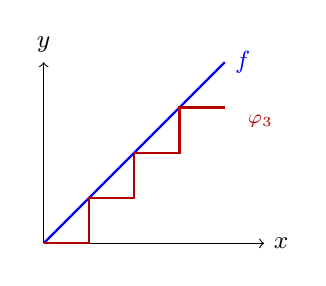
\begin{tikzpicture}[scale=1.0]
\draw[->] (0,0) -- (2.8,0) node[right] {\small $x$};
\draw[->] (0,0) -- (0,2.3) node[above] {\small $y$};
\draw[thick, blue] (0,0) -- (2.3,2.3) node[right] {\small $f$};
\draw[thick, red!70!black]
  (0,0) -- (0.575,0) -- (0.575,0.575) -- (1.15,0.575) -- (1.15,1.15) -- (1.725,1.15) -- (1.725,1.725) -- (2.3,1.725);
\node[red!70!black] at (2.75,1.55) {\scriptsize $\varphi_3$};
\end{tikzpicture}
\end{center}
\end{thm}

\pause

\begin{remark}
按 $y$ 轴的\alert{二进分割}作阶梯: 对固定的 $n$, 以步长 $2^{-n}$ 从下往上``垫台阶'', 高度封顶在 $n$; $n \to \infty$ 时台阶无限加密、封顶升高.
\end{remark}

\end{frame}

%------------------------------------------------

\begin{frame}{逼近定理的证明 (一): 构造与单调性}

\startproof[bg=yellow, fg=red](证明)
对每个 $n \in \mathbb{N}$, 定义简单函数
\[
\varphi_n(x) =
\begin{cases}
\dfrac{r-1}{2^n}, & \text{若 } \dfrac{r-1}{2^n} \leqslant f(x) < \dfrac{r}{2^n}, \quad r = 1, 2, \ldots, n2^n, \\[2mm]
n, & \text{若 } f(x) \geqslant n.
\end{cases}
\]
(诸水平集 $E\big(\frac{r-1}{2^n} \leqslant f < \frac{r}{2^n}\big)$ 可测, 故 $\varphi_n$ 是简单函数.)

\pause

\textbf{单调性}: 设 $k > n$.
若 $\frac{r-1}{2^n} \leqslant f(x) < \frac{r}{2^n}$, 则 $\frac{r-1}{2^n} = \frac{2^{k-n}(r-1)}{2^k}$, 故
\[
\varphi_k(x) \geqslant \frac{2^{k-n}(r-1)}{2^k} = \frac{r-1}{2^n} = \varphi_n(x);
\]
若 $f(x) \geqslant n = \frac{2^k \cdot n}{2^k}$, 则 $\varphi_k(x) \geqslant \frac{2^k \cdot n}{2^k} = n = \varphi_n(x)$.

所以 $\varphi_n(x) \leqslant \varphi_k(x) \leqslant f(x)$, $\forall\, k > n$.
\qed

\end{frame}

%------------------------------------------------

\begin{frame}{逼近定理的证明 (二): 收敛}

\startproof[bg=yellow, fg=red](证明 (续): $\varphi_n(x) \to f(x)$)
\textbf{1$^\circ$} 若 $f(x) < +\infty$, 即 $f(x) \in \mathbb{R}$, 取 $N = \lfloor f(x) \rfloor + 1 \in \mathbb{N}$, 则 $f(x) < N$. 于是对 $n > N$, $f(x)$ 落入某个长度为 $2^{-n}$ 的左闭右开区间,
\[
0 \leqslant f(x) - \varphi_n(x) \leqslant \frac{1}{2^n} \longrightarrow 0,
\qquad \text{故} \lim_{n \to \infty} \varphi_n(x) = f(x).
\]

\pause

\textbf{2$^\circ$} 若 $f(x) = +\infty$, 则 $\forall\, n$, $f(x) > n$, 故 $\varphi_n(x) = n$, 从而 $\lim_n \varphi_n(x) = \lim_n n = +\infty = f(x)$.
\qed

\pause

\begin{attnblock}
``可测函数 = 递增简单函数列的极限''. 这是连接函数与集合 (测度) 的桥梁: 第四章的积分将\alert{先对简单函数定义}, 再沿这条定理推广.
\end{attnblock}

\end{frame}

%------------------------------------------------

\begin{frame}{注记: 三种常用的变体}

\begin{enumerate}
\item \textbf{一般可测函数}: $f = f_+ - f_-$, 分别对 $f_+$、$f_-$ 用逼近定理, 得非负递增简单函数列 $\{\varphi_n\}$、$\{\psi_n\}$ 使 $f_+ = \lim \varphi_n$、$f_- = \lim \psi_n$, 于是
\[
f = \lim_{n \to \infty} \big(\varphi_n(x) - \psi_n(x)\big)
\]
(两个简单函数之差的极限; $f$ \alert{有界}时收敛还是一致的 --- 将在 \S 4 中用到);
\pause
\item \textbf{特征函数级数}: 设 $f$ 非负可测, $\varphi_n \uparrow f$, 令 $\varphi_0 = 0$、$\tau_n = \varphi_n - \varphi_{n-1}$ (非负简单函数), 则
\[
f = \sum_{n=1}^{\infty} \tau_n = \sum_{n=1}^{\infty} \sum_{k} c_{n,k}\, \chi_{E(\tau_n = c_{n,k})}
\]
--- \alert{非负可测函数 = 可测集特征函数的非负级数};
\pause
\item \textbf{截断}: 再取 $\psi_n(x) = \varphi_n(x) \cdot \chi_{E \cap [-n, n]}(x)$, 则 $0 \leqslant \psi_1 \leqslant \psi_2 \leqslant \cdots$, $\lim_n \psi_n(x) = f(x)$, 且每个 $\psi_n$ \alert{具有紧支集} (对 $E \subset \mathbb{R}$).
\end{enumerate}

\end{frame}

%------------------------------------------------

\section[小结]{小结与展望}

%------------------------------------------------

\begin{frame}{小结}

\begin{itemize}
\item \textbf{可测函数}: $E(f>\alpha)$ 可测 ($\forall\, \alpha$); 等价水平集族众多; 连续函数 $\Rightarrow$ 可测;
\pause
\item \textbf{验证工具箱}: 简单函数可测; 稠密集判别法 (取 $\mathbb{Q}$); 限制与拼接;
\pause
\item \textbf{运算与极限}: 四则可测 (有理数分裂); $\sup/\inf/\varlimsup/\varliminf$ 可测; 逐点 (或 a.e.) 极限可测; 正负部与 $|f|$ 可测;
\pause
\item \textbf{a.e.\ 语言}: 命题在零测集外成立即可 --- 可测函数类对 a.e.\ 相等封闭 ($f \sim g$, $g$ 可测 $\Rightarrow f$ 可测);
\pause
\item \textbf{简单函数逼近}: 非负可测 $f$ $\Longleftarrow$ 递增简单函数列 (二进分割台阶); 变体: 差的极限、特征函数级数、紧支集截断.
\end{itemize}

\end{frame}

%------------------------------------------------

\begin{frame}{展望}

\begin{itemize}
\item \textbf{\S 3.2 可测函数列的收敛性}: 逐点收敛之外, 还有\alert{几乎处处收敛、近一致收敛 (Egorov)、依测度收敛 (Riesz)} 等层次及其互相刻画;
\pause
\item \textbf{\S 3.3 可测函数的构造}: Luzin 定理 --- 可测函数``去掉小测度集后连续'', 即 \alert{可测 $\approx$ 连续};
\pause
\item \textbf{\S 4 勒贝格积分}: $\displaystyle\int f = \lim \int \varphi_n$ (简单函数逼近定理正是定义积分的跳板), Dirichlet 函数将变为可积且积分为 $0$.
\end{itemize}

\end{frame}

%------------------------------------------------

\ifIncludeExercise
\begin{frame}{作业}

\begin{block}{教材第三章 §3.1 习题}
\begin{itemize}
\item \textbf{2.} 证明: $f$ 是 $E$ 上可测函数的充要条件是, 对任一有理数 $r$, 集 $E(f > r)$ 恒可测. 又问: 若假设对任一有理数 $r$, 集 $E(f = r)$ 恒可测, $f$ 是否一定可测?
\item \textbf{4.} 设 $f$ 是 $E$ 上的可测函数, $G, F$ 分别为 $\mathbb{R}$ 中的开集与闭集. 试问 $E(f \in G)$ 与 $E(f \in F)$ 是否可测? (记号 $E(f \in A) = \{x \in E:\ f(x) \in A\}$.)
\item \textbf{7.} 设 $f(x)$ 是 $(-\infty, +\infty)$ 上的连续函数, $g(x)$ 是 $[a,b]$ 上的有限可测函数, 证明 $f(g(x))$ 是可测函数.
\item \textbf{10.} 设 $x \in [0,1)$ 的三进表示为 $x = 0.x_1 x_2 \cdots$ ($x_k \in \{0,1,2\}$, 约定不用循环节全 $2$ 的表示), $P_i$ 表示三进表示中不出现数字 $i$ 的点集 ($i = 0, 1, 2$). 令
$f(x) = x + i$ (当 $x \in P_i$, $i = 0, 1, 2$), $f(x) = x + 3$ (当 $x \in [0,1) \setminus \bigcup_i P_i$), 并规定 $f(0) = 3$, $f(1/2) = 7/2$. 问 $f$ 是否可测? 是否连续?
\item \textbf{11.} 设 $f(x,y)$ 是 $\mathbb{R}^2$ 上几乎处处有限的函数, 对每个固定的 $x$ 关于 $y$ 连续, 对每个固定的 $y$ 关于 $x$ 也连续. 试证 $f(x,y)$ 是 $\mathbb{R}^2$ 上的可测函数.
\end{itemize}
\end{block}

\end{frame}
\fi

%------------------------------------------------

\end{document}
